\documentclass[12pt]{extarticle}
\usepackage[english,ukrainian]{babel}
\usepackage[utf8]{inputenc}
\usepackage{amsmath,amssymb}
\usepackage{parskip}
\usepackage{graphicx}
\usepackage{xcolor}
\usepackage{tcolorbox}
\tcbuselibrary{skins}
\usepackage[framemethod=tikz]{mdframed}
\usepackage{chngcntr}
\usepackage{enumitem}
\usepackage{hyperref}
\usepackage{float}
\usepackage{subfig}
\usepackage{esint}
\usepackage[top=2.5cm, left=3cm, right=3cm, bottom=4.0cm]{geometry}
\usepackage[table]{xcolor}
\usepackage{algorithm}
\usepackage{algpseudocode}
\usepackage{listings}
\usepackage{xcolor}

\title{Домашня робота \#1 з курсу ``Комплексний аналіз'' (частина перша)}
\author{Студента 3 курсу групи МП-31 Захарова Дмитра}
\date{\today}

\begin{document}

\maketitle

\section*{Завдання 1.} 

\textbf{Умова.} Зобразити на площині ($z \in \mathbb{C}$):
\[
\text{Re}\, \frac{z-1}{z+1} = 0
\]

\textbf{Розв'язок.} Нехай $z = x+i y$ де $x,y \in \mathbb{R}$. Розглянемо
\[
w = \frac{z-1}{z+1}
\]

та запишемо дійсну частину цього виразу. Маємо:
\[
w = \frac{x + iy - 1}{x + iy + 1} = \frac{(x+iy-1)(x+1-iy)}{(x+1)^2 + y^2}
\]

Розкриваємо дужки так, щоб отримати лише дійсні компоненти:
\[
\text{Re} \, w = \frac{x^2+x+y^2-x-1}{(x+1)^2+y^2} = \frac{x^2+y^2-1}{(x+1)^2+y^2}
\]

Нам потрібно знайти набір точок $\{(x,y) \in \mathbb{R}^2: \text{Re} \, w = 0\}$, тобто по суті знайти розв'язок:
\[
\frac{x^2+y^2-1}{(x+1)^2+y^2} = 0
\]

Помітимо, що вираз зліва визначений на $\mathbb{R}^2 \setminus \{(-1,0)\}$. Для інших точок:
\[
x^2+y^2-1 = 0,
\]

що є рівнянням одиничного кола. Оскільки $(-1,0)$ йому належить, то відповіддю є одиничне коле з виколотою точкою $(-1,0)$ (див. рис. \ref{fig:1}).

\begin{figure}[H]
    \centering
    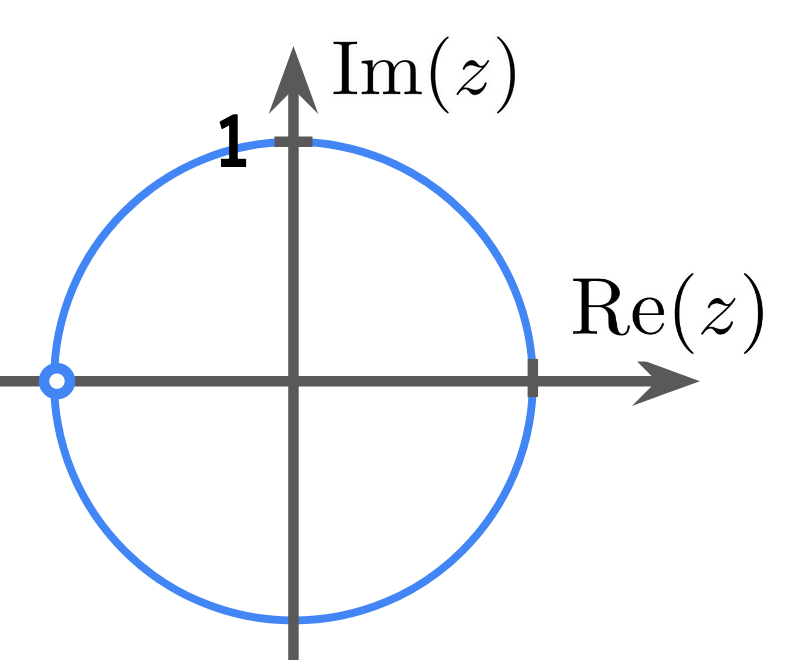
\includegraphics[width=0.4\textwidth]{images/hw_1/hw_1_1.png}
    \caption{Множина $\{z \in \mathbb{C}: |z|=1\} \setminus \{-1\}$}
    \label{fig:1}
\end{figure}
\vspace{5px}

\textbf{Відповідь.} Дивись рис. $\ref{fig:1}$

\section*{Завдання 2.} 

\textbf{Умова.} Знайти дійсну та уявну частину наступних комплексних чисел:
\begin{enumerate}
    \item $\left(\frac{i^5+2}{i^{19}+1}\right)^2$
    \item $\frac{(1+i)^5}{(1-i)^3}$
\end{enumerate}

\textbf{Розв'язок.} 

\textit{Пункт 1.} Помітимо, що $i^5=(i^4)\cdot i = i$ і також $i^{19}=i^{16} \cdot i^3 = -i$. Тому:
\[
\left(\frac{i^5+2}{i^{19}+1}\right)^2 = \left(\frac{2+i}{1-i}\right)^2
\]

Вираз під квадратом множимо та ділимо на $1+i$:
\[
\left(\frac{2+i}{1-i}\right)^2 = \left(\frac{(2+i)(1+i)}{2}\right)^2 = \frac{1}{4}(1+3i)^2 = \frac{-8+6i}{4} = -2 + \frac{3}{2}i
\]

\textit{Пункт 2.} Помічаємо, що $1+i=\sqrt{2}e^{i\pi/4}$, а $1-i=\sqrt{2}e^{-i\pi /4 }$. Тому:
\[
\frac{(1+i)^5}{(1-i)^{3}} = \frac{2^{5/2}e^{5i\pi/4}}{2^{3/2}e^{-3i\pi/4}} = 2 e^{2i\pi} = 2
\]

\textbf{Відповідь.} 

1. Дійсна частина $-2$, уявна $3/2$.

2. Дійсна частина $2$, уявна $0$.

\section*{Завдання 3.}

\textbf{Умова.} Зобразити на площині $z \in \mathbb{C}$, якщо:

\begin{enumerate}
    \item $|z-i| > 1$
    \item $0 < |z+i| < 2$
\end{enumerate}

\textbf{Розв'язок.} 

\textit{Пункт 1.} $|z-i|=1$ є колом з центром у $(0,1)$ радіуса $1$, отже $|z-i|>1$ є увесь простір $\mathbb{C}$ мінус закрашене з границею куля.

\textit{Пункт 2.} $|z+i|=2$ є колом з центром у $(0,-1)$ радіуса $2$, а $|z+i|=0$ просто точкою $(0,-1)$. Отже, шукана множина -- це зафарбована відкрита куля з виколотим центром.

\begin{figure}[H]
    \centering
    \subfloat[\centering $|z-i|>1$]{{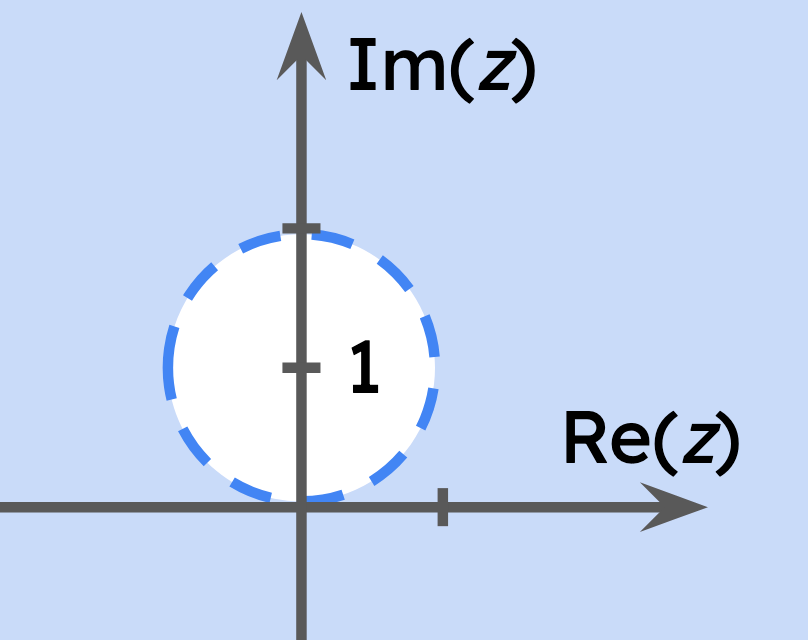
\includegraphics[width=5cm]{images/hw_1/hw_1_3-1.png} }}%
    \qquad
    \subfloat[\centering $0<|z+i|<2$]{{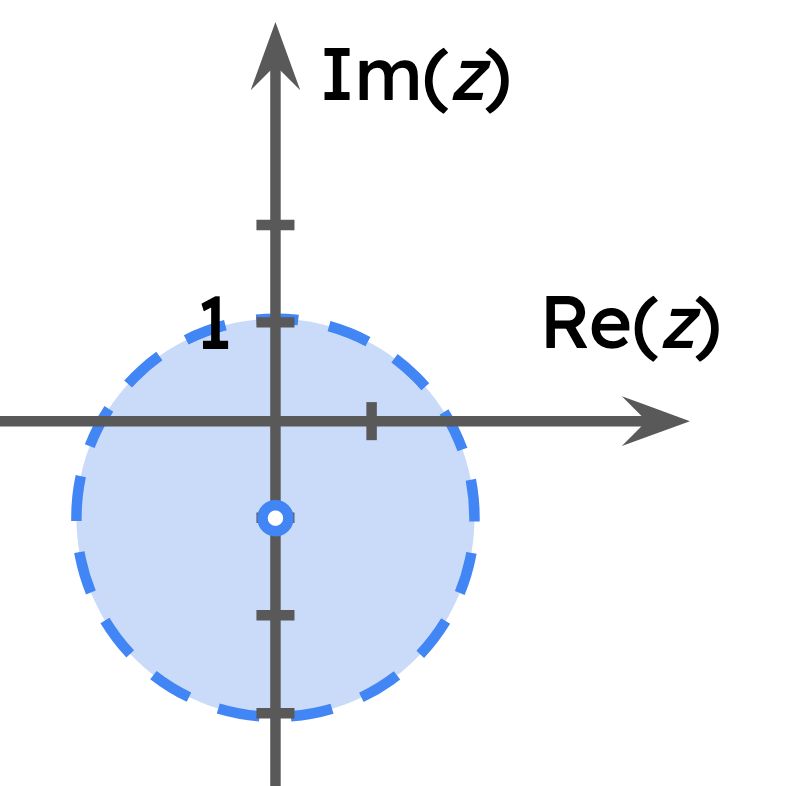
\includegraphics[width=5cm]{images/hw_1/hw_1_3-2.png} }}%
    \caption{Відповіді на задачі $3.1$ та $3.2$}%
    \label{fig:3}%
\end{figure}

\textbf{Відповідь.} Дивись рис. \ref{fig:3}.

\end{document}

